% !Mode:: "TeX::UTF-8"
\documentclass[myposter,portrait]{sciposter}

%% uzitocne package
\usepackage{multicol}
\usepackage{color}
\usepackage{graphicx}
\usepackage{tikz}
\usetikzlibrary{arrows,backgrounds,fit,positioning,trees}

%% znaky s diakritikou
\usepackage[utf8]{inputenc}
\usepackage[T1]{fontenc}
% \usepackage[slovak]{babel} % slovenske delenie slov

%% definicia farieb
\definecolor{mainCol}{rgb}{0.91,0.82,0.74} % farba pozadia posteru
%\definecolor{mainCol}{rgb}{1,1,1} % farba pozadia posteru
\definecolor{sectionCol}{rgb}{0,0,0} % farba nadpisu
\definecolor{textCol}{rgb}{0.2,0,0} % farba hlavneho textu
\definecolor{BoxCol}{rgb}{1,1,0.8} % farba boxu okolo nadpisov

\def\mysection#1{
{\color{sectionCol}\section*{\sc\bfseries #1}}}

\begin{document}
\setlength{\logowidth}{20cm}
\setlength{\titlewidth}{\textwidth}
\addtolength{\titlewidth}{-\logowidth}
\rightlogo[0.9]{fmfilogo-farebne}
\useleftlogofalse

\color{textCol}

\title{Membrane computing}
\author{Michal Kováč\\
        Supervisor: Damas Gruska}
\institute{%
Katedra aplikovanej informatiky,
FMFI UK, Mlynská Dolina, 842~48~Bratislava\\
}
\maketitle

\begin{multicols*}{3}

\mysection{Introduction}


Well established computation models motivated by biology such as neural networks and evolutionary algorithms has already proven that it is worth to be inspired by biology.

\vspace{10mm}
\includegraphics[width=0.3\columnwidth]{neural}
\hspace{0.1\columnwidth}
\includegraphics[width=0.6\columnwidth]{evolution}
\vspace{10mm}

Other emerging areas are still awaiting for their more significant uses. One of them is the membrane computing. It is relatively young field of natural computing - in comparison: neural networks have been researched since 1943 and membrane systems since 1998\cite{Paun98}.

Membrane systems are distributed parallel computing devices inspired by the structure and functionality of cells. Recently, many variants have been developed in order to simulate cells more realistically or just to improve the computational power.

\vspace{10mm}
\includegraphics[width=\columnwidth]{wallpaper}

\mysection{Membrane structure}
Biological systems usually have hierarchical structure where objects and information flows between regions, what can be interpreted as a computation process.

\vfill
\columnbreak

This hierarchical structure can be also interpreted as rooted tree as seen on the figures 1 and 2. The objects are stored in the tree nodes and can be sent through the edges.

\vspace{10mm}

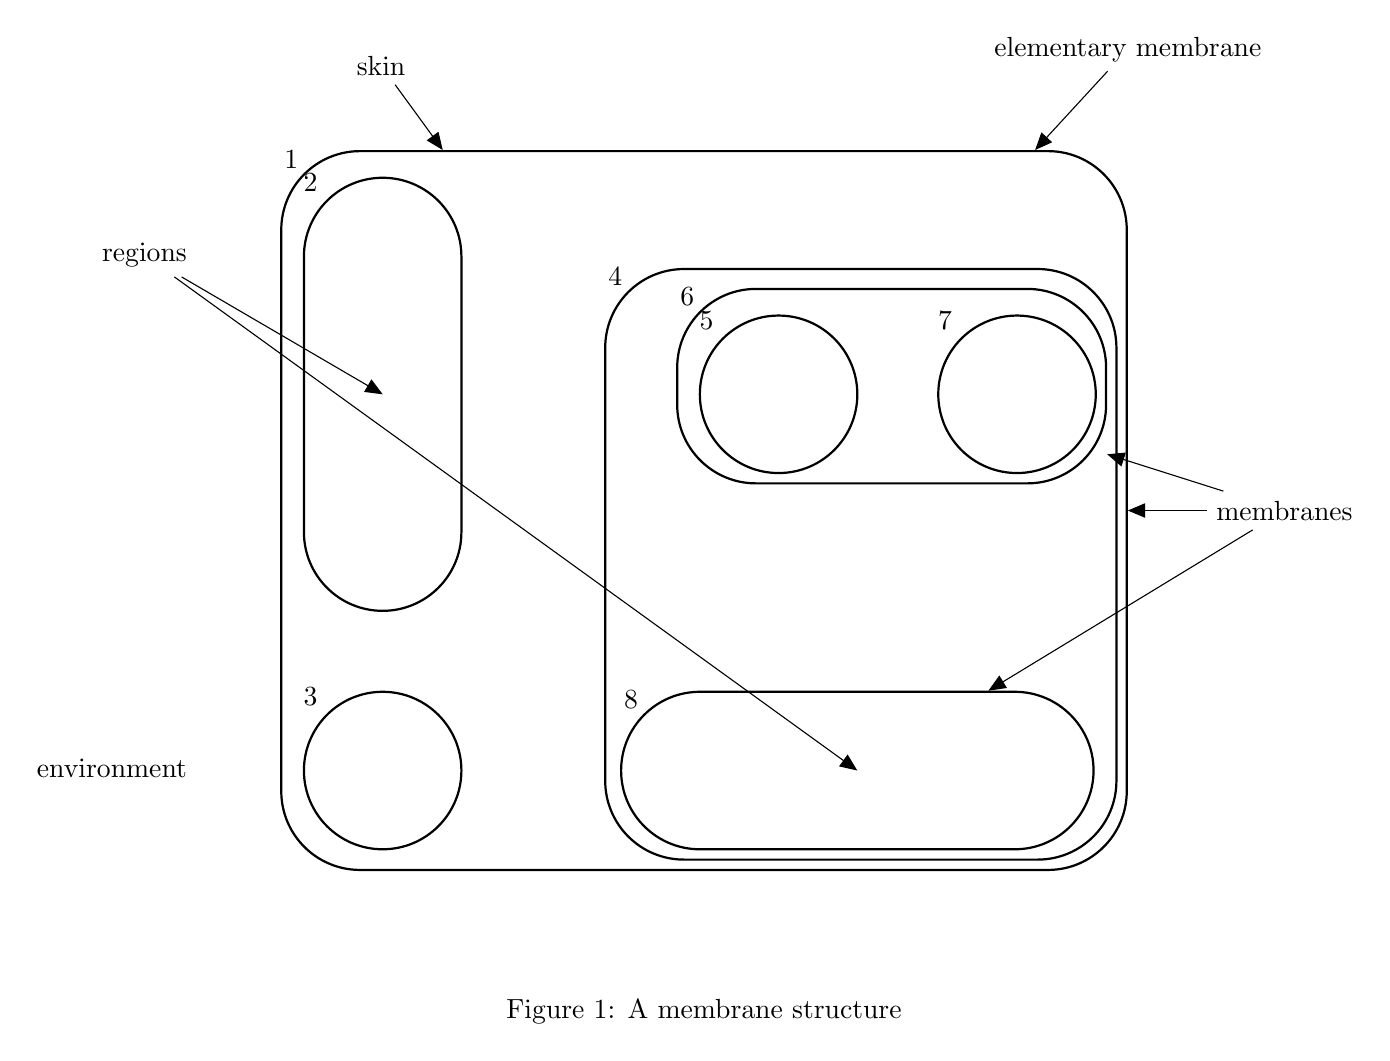
\begin{tikzpicture}[node distance=2mm,-triangle 45,line width=1mm]
  \tikzstyle{label of} = [above left=-5mm of #1]
  \tikzstyle{membrane} = [draw,thick,rounded corners=1cm,minimum width=2cm,minimum height=2cm,rectangle]
  \node [membrane,minimum height=55mm] (m2) {};
  \node [label of=m2] (l2) {2};
  \node [membrane,below=1cm of m2] (m3) {};
  \node [label of=m3] (l3) {3};
  
  \node [membrane,right=3cm of m2] (m5) {};
  \node [label of=m5] (l5) {5};  
  \node [membrane,right=1cm of m5] (m7) {};
  \node [label of=m7] (l7) {7};

  \begin{pgfonlayer}{background}
    \node [membrane,fit=(m5)(l5)(m7)(l7)] (m6) {};
  \end{pgfonlayer}
  \node [label of=m6] (l6) {6};

  \node [membrane,right=2cm of m3,minimum width=6cm] (m8) {};
  \node [label of=m8] (l8) {8};

  \begin{pgfonlayer}{background}
    \node [membrane,fit=(m6)(l6)(m8)(l8)] (m4) {};
  \end{pgfonlayer}
  \node [label of=m4] (l4) {4};
  
  \begin{pgfonlayer}{background}
    \node [membrane,fit=(m2)(l2)(m3)(l3)(m4)(l4)] (m1) {};
  \end{pgfonlayer}
  \node [label of=m1] (l1) {1};

  \node [above right=1cm of l1.north] (skin) {skin}
    edge (m1);
  \node [above=1cm of m1.north east] (elementary membrane) {elementary membrane}
    edge (m1);
  \node [right=1cm of m1.east] (membranes) {membranes}
    edge (m6)
    edge (m8)
    edge (m1);
  \node [below=1.5cm of m1] (figure) {Figure 1: A membrane structure};
  \node [above left=1.5cm of m1.south west] (environment) {environment};
  \node [below left=1.5cm of m1.north west] (regions) {regions}
    edge (m2.center)
    edge (m8.center);

\end{tikzpicture}

\begin{tikzpicture}[level distance=4cm,sibling distance=4cm]
  \tikzstyle{every node} = [circle,draw]

  \node (Root) {1}
    child { node {2} }
    child { node {3} }
    child {
      node {4}
      child {
        node {6}
        child {
          node (n5) {5}
        }
        child {
          node {7}
        }
      }
      child { node {8} }
    };
  \node [draw=none,rectangle,below=0.5cm of n5] {Figure 2: The tree describing the membrane structure from Figure 1};

\end{tikzpicture}

\mysection{P systems}

Membranes and regions delimited by them has clearly 1:1 correspondence. Each region contains a multiset of objects. These objects can evolve according to evolution rules which are associated with membranes. Evolution rules are applied in a maximally parallel manner - in each step, a maximal multiset of rules is nondeterministically chosen and applied.

This computing device is called P system\footnote{P in P systems stands for surname of it's founder Gheorghe P\u aun.} and is Turing complete.

Next figure demonstrates a computation of a P system for Fibonacci numbers.

\mysection{Variants}

Since the first publication in 1998, huge amount of variants has been proposed. Some of them are Turing complete, others are not. Maximal parallelismus is one of the most questioned attribute. P systems in sequential mode are not Turing complete. Various combinations of variants have been studied and some of them have been shown Turing complete also in sequential mode.

\mysection{Inhibitors}

One of the variants is P system with inhibitors. Some of the objects (inhibitors) can be used in evolution rules such that their presence in the region prevents the application of the rule. One of our results is the proof that sequential P systems with inhibitors are Turing complete. It is proven by simulation of the maximally parallel P system, which is Turing complete. The challenging part was the simulation of maximally parallel step.


\mysection{SAT in linear time}

Linear time solutions to NP-complete problems by means of P systems are achieved by trading time (number of computation steps) for space (number of membranes and objects). This is inspired by the capabililty of cells to produce an exponential number of new membranes in linear time.

However, many simulators of P system are inefficient since they cannot handle the parallelism of these devices. Nowadays, we are witnessing the consolidation of the GPUs as a parallel framework to compute general purpose applications. The simulation of P systems with active membranes using GPUs is analysed in \cite{Cecilia10} and an efficient linear solution to the SAT problem is illustrated.

\mysection{P system computing Fibonacci sequence}

\vspace{10mm}
\includegraphics[width=\columnwidth]{p_system_fibonacci}
\vspace{10mm}


%% zoznam literatury
\bibliographystyle{apalike}
\bibliography{references}

\end{multicols*}
\end{document}

